\chapter{Métodos}\label{chapter:Metodos}
En este capítulo se detallan los criterios seguidos para la elección de la geometría de los espaciadores y su escala, los cálculos realizados para adaptar las propiedades de los materiales a las limitaciones de escala de los programas de simulación, los procedimientos seguidos para realizar las simulaciones y el procedimiento seguido para la extracción de los datos de la simulación de CFD.
\section{Criterios de geometría y escala}
Los criterios de geometría y escala se basan principalmente en el proceso de fabricación de los nano-espaciadores por fotolitografía, que es la técnica que se utilizará en el desarrollo de los primeros experimentos que intentarán corroborar los resultados obtenidos en este trabajo de simulación, esto en una siguiente etapa de la investigación.\\\\
La base del nano-espaciador es cuadrada por ser la geometría más sencilla de fabricar mediante procesos fotolitográficos y para realizar cálculos, por ser sus ecuaciones de área y volumen las más sencilla de los polígonos regulares cerrados. El lado de la base del nano-espaciador son de 3 $\mu m$ por ser el límite de resolución de la mayoría de equipos de fotolitografía, es decir, es la mínima distancia que se puede definir mediante fotolitografía.\\\\
Se utiliza 100 nm como la distancia mínima para definir la altura mínima de los nano-espaciadores, correspondiente a 1 mm de la escala del modelo 3D en Inventor. Por lo tanto, el factor de escala que se aplica a las unidades de longitud es $10^4$, que se toma en cuenta a la hora de definir las propiedades térmicas que involucren unidades de longitud, como es la conductividad térmica ($W/m2$).
%%% CALCULOS DE LAS PROPIEDADES DE LOS MATERIALES
\section{Cálculos de las propiedades de los materiales para las simulaciones}
Para obtener los nuevos parámetros de distancias, áreas y volúmenes del modelo 3D del nano-espaciador se procede a obtener las relaciones de escala entre el modelo y la realidad. También se obtienen las relaciones de las propiedades más significativas de los materiales de la realidad y las simulaciones de transmisión de calor por conducción, siendo la principal propiedad la conductividad térmica. Otras propiedades que se toman en cuenta son la densidad y el calor específico, teniendo que destacar la resistencia de contacto por unidad de área entre el nano-espaciador y el emisor.\\\\
Para diferenciar las dimensiones reales de las dimensiones utilizadas en el modelo 3D se utilizará el apostrofe después de la variable correspondiente, por ejemplo, para la longitud real se usa $L$ y para la longitud en el modelo 3D se usa $L'$.\\\\
La relación de longitudes entre el modelo 3D y la realidad es:
\begin{equation}
{L'}/{L}={1mm}/{100nm}=10^4
\label{eq:relacion_longitud}
\end{equation}
%%%  AREA
\subsection{Área}
La sección de los nano-espaciadores es un cuadrado cuya fórmula de área es $A=L^2$, donde $A$ es el área y $L$ el lado del cuadrado, siendo la relación de las áreas la siguiente:
\begin{equation}
	\dfrac{A'}{A}=\left(\dfrac{L'}{L}\right)^2=10^8
	\label{eq:relacion_areas}
\end{equation}
%%% VOLUMEN
\subsection{Volumen}
El volumen de un prisma de base cuadrada se expresa como $V=A\cdot L$, donde $L$ es la altura del prisma.
\begin{equation}
	\dfrac{V'}{V}=\dfrac{A'\cdot L'}{A\cdot L} = 
	\dfrac{A'}{A}\cdot \dfrac{L'}{L} \ \Longrightarrow \ \dfrac{V'}{V} =10^{12}
	\label{eq:relacion_volumen}
\end{equation}
El volumen de cada nano-espaciador en el modelo será $10^{12}$ veces el volumen original.
%%% DENSIDAD
\subsection{Densidad}
La masa de cada elemento es igual entre el modelo($M'$) y la realidad($M$), por lo tanto la densidad varía.
\begin{equation}
\dfrac{\rho '}{\rho}=\dfrac{M'/V'}{M/V}=\dfrac{M'}{M}\cdot \dfrac{V}{V'} \ \Longrightarrow \ 
\dfrac{\rho '}{\rho}=10^{-12}
\label{eq:relacion_densidad}
\end{equation}
La densidad de cada elemento en el modelo será $10^{-12}$ veces la densidad de la realidad.
%%% CONDUCTIVIDAD TERMICA
\subsection{Conductividad Térmica}
La resistencia térmica de los materiales del modelo de simulación se mantiene igual a la de la realidad, por lo tanto, la conductividad térmica de los materiales en el modelo son distintas a la realidad. Sabiendo que la fórmula de la resistencia térmica de conducción es $R=1/k \cdot L/A$, donde $k$ es la conductividad térmica, $L$ la longitud y $A$ es la sección, se puede obtener la relación de las conductividades térmicas del modelo de simulación respecto a la realidad.
\[ \dfrac{R}{R'}= \dfrac{1/k}{1/k'}\cdot \dfrac{L/A}{L'/A'}= \dfrac{k'}{k}\cdot \dfrac{L}{L'}\cdot \dfrac{A'}{A}=1\]
\begin{equation}
\dfrac{k'}{k}=\dfrac{L'}{L}\cdot \dfrac{A}{A'}=\dfrac{10^4}{10^8} \ \Longrightarrow \ \dfrac{k'}{k}=10^{-4}
\label{eq:relacion_conductividadTermica}
\end{equation}
Para el caso del nano-espaciador de $SiO_2$ que puede presentar diferentes porosidades para el material, se multiplica la conductividad térmica por la conductividad térmica normalizada para dicha porosidad \cite{ThermalConductivity_SiO2_2018}.
%%% CALOR ESPECIFICO
\subsection{Calor Específico}
El calor específico de los materiales del modelo de simulación es el mismo que el de la realidad porque el calor específico se define como la cantidad de calor necesaria que hay que suministrar a una unidad de masa para elevar su temperatura en una unidad, como la masa del modelo de simulación es igual a la de la realidad, la cantidad de energía necesaria para elevar una unidad de temperatura va a ser igual al del modelo de simulación respecto a la realidad, por lo tanto, el calor específico se mantiene igual al de la realidad.
%%% RESISTENCIA DE CONTACTO
\subsection{Resistencia de contacto}\label{sec:metodos_Rc}
La resistencia de contacto ($R_c$) es difícil de modelar matemáticamente en una ecuación ya que depende de muchas variables, como la temperatura, presión, entre otros. La resistencia de térmica producida por la resistencia de contacto es $R_{th}=R_{c}/A$, donde A es la superficie de contacto, por lo tanto se ve afectado por la diferencia de escala entre el modelo de simulación y la realidad.
\[ \dfrac{R_{th}'}{R_{th}}=\dfrac{R_c'}{R_c}\cdot \dfrac{A}{A'}=1 \]
\begin{equation}
	\dfrac{R_{th}'}{R_{th}}=\dfrac{R_c'}{R_c}\cdot \dfrac{A}{A'}=1 \ \Longrightarrow \  \dfrac{R_c'}{R_c}=\dfrac{A'}{A}=10^8
	\label{eq:relacion_Rc}
\end{equation}
%%% YOVANOVICH
Para los casos que el emisor de la \acrshort{nptc} sea de \gls{ss}, la $R_c$ es obtenida a través de la conductancia de contacto (\gls{hc}) según un modelo matemático \cite{experimental_Rc_SS}, y según la ecuación de Cooper reducida por Yovanovich (ecuación \eqref{eq:modeloYovanovich}).

\begin{subequations}
\begin{equation}
\dfrac{P}{H_c}=\left[ \dfrac{P}{c_1\left(1.62\sigma/m\right)^{c_2}} \right]^{\frac{1}{2+0.071c_2}}
\label{eq:modeloYovanovich}
\end{equation}
\begin{equation}
\dfrac{h_c\sigma}{k_sm}=1.25\left(\dfrac{P}{H_c}\right)^{0.95}
\label{eq:correlacionCooperSimplificadaYovanovich}
\end{equation}
\label{eqs:ecuacionesRcYovanovich}
\end{subequations}

%% Valores de las constantes
Donde $c_1$ es 10.6 GPa, $c_2$ es -0.40, $\sigma$ es la combinación RMS de la rugosidad de ambas superficies de los materiales con $\sigma_i$ siendo la rugosidad de la superficie $i$ (ecuación \eqref{eq:sigmaRMS}), $m$ es la combinación RMS de la media absoluta de la pendiente de la rugosidad con $m_i$ siendo la media de la pendiente absoluta de la superficie $i$ (ecuación \eqref{eq:mRMS}), $k_s$ es la media armónica de la conductividad térmica con $k_i$ siendo la conductividad térmica del material $i$ (ecuación \eqref{eq:condArmonica}), $H_c$ es la micro-dureza Vickers del material más duro y P es la presión aplicada.
\begin{subequations}
\begin{minipage}{0.29\textwidth}
\begin{equation}
m=\sqrt{m_1^2+m_2^2}
\label{eq:mRMS}
\end{equation}
\end{minipage}
\hfill
\begin{minipage}{0.28\textwidth}
\begin{equation}
\sigma=\sqrt{\sigma_1^2+\sigma_2^2}
\label{eq:sigmaRMS}
\end{equation}
\end{minipage}
\hfill
\begin{minipage}{0.28\textwidth}
\begin{equation}
k_s=2\cdot \frac{k_1\cdot k_2}{k_1+k_2}
\label{eq:condArmonica}
\end{equation}
\end{minipage}
\label{eqs:RMS}
\end{subequations}
Estas son las únicas expresiones analíticas que se han encontrado en la literatura para calcular la \gls{hc} entre dos superficies, las cuales han sido validadas para el caso concreto de dos superficies de acero inoxidable 304 (SS) \cite{experimental_Rc_SS}. Para tener una mejor idea como la resistencia de contacto afecta a la conducción de calor simplificamos las ecuaciones suponiendo que el nano-espaciador de $SiO_2$ es liso, por ende, su $m_i$ y su $\sigma_i$ son nulas. Por lo tanto, se calcula la relación de las ecuaciones para el caso de los dos aceros y para el caso de SS-$SiO_2$.\\\\
Como se puede observar en las ecuaciones \ref{eqs:ecuacionesRcYovanovich}, el valor de $\sigma$ y $m$ se presentan siempre relacionados como $\sigma / m$, y se cumple que $\sigma /m =\sigma ' / m'$ porque al suponer que el caso de dos aceros tienen idénticas $m_i$ y $\sigma_i$, la relación $\sigma / m$ queda como $\sigma_i / m_i$, que resulta ser la misma relación para el caso de SS-$SiO_2$.\\\\
\[ \frac{\sigma}{m}=\frac{\sqrt{\sigma_{SS}^2+\sigma_{SS}^2}}{\sqrt{m_{SS}^2+m_{SS}^2}}=\frac{\sigma_{SS}\sqrt{2}}{m_{SS}\sqrt{2}} =\frac{\sigma_{SS}}{m_{SS}}\]
\[ \frac{\sigma'}{m'}=\frac{\sqrt{\sigma_{SS}^2+0^2}}{\sqrt{m_{SS}^2+0^2}}=\frac{\sigma_{SS}}{m_{SS}} \]
Por lo tanto, considerando que $c_1$ y $c_2$ no varían con el cambio de material la relación de $h_c'$ respecto a \gls{hc} se obtiene relacionando la ecuación \eqref{eq:correlacionCooperSimplificadaYovanovich} del modelo a simular con la realidad.
\[Cte=1.25\frac{m}{\sigma}\cdot \left(\dfrac{P}{H_c}\right)^{0.95} \qquad \Longrightarrow \qquad h_c=k_s\cdot Cte\]
Donde $Cte$ es una constante que es igual para el caso de los aceros y el caso SS-$SiO_2$. El valor de $k_s$ para el caso de de los aceros es $k_{SS}$, siendo $k_{SS}$ la conductividad térmica del acero inoxidable 304. 
\[ \frac{h_c'}{h_c}=\frac{k_s'}{k_s}\cdot \frac{Cte}{Cte}=\frac{2 \cdot \frac{k_{SS}\cdot k_{SiO_2}}{k_{SS}+k_{SiO_2}}}{k_{SS}}\]
\begin{equation}
\frac{h_c'}{h_c}=2\cdot \frac{k_{SiO_2}}{k_{SS}+k_{SiO_2}}
\label{eq:relacion_conductividadesTermicas}
\end{equation}
Para este trabajo los datos utilizados de las conductividades térmicas de los materiales para la relación de las conductancias de contacto son a temperatura ambiente, el valor de $k_{SiO_2}$ es $1.5 \ W/\left( m^2 K\right)$ y el valor de $k_{SS}$ es de $15 \ W/\left( m^2 K\right)$, quedando la relación de conductancias de contacto como ${h_c'}/{h_c}=0.1818$.

%%%%%%%%     PROCEDIMIENTOS DE LAS SIMULACIONES Y EXTRACCION DE RESULTADOS
\section{Procedimientos de las simulaciones y extracción de resultados}
A continuación se describen los procedimientos seguidos en este trabajo para la realización de la simulación de la transmisión de calor por radiación de campo cercano, la simulación de la transmisión de calor por conducción y la extracción de los datos de las simulaciones.\\
\subsection{Para la radiación de campo cercano}
%Aquí tendrías que meter las simulaciones de campo cercano y hablar del método (está descrito en un paper que te pasé
Las simulaciones de transmisión de calor por radiación de campo cercano se realizan para una combinación de varios materiales de emisor y célula en un rango de distancias de 100nm a 1000nm. Para la realización de las simulaciones y la obtención de la potencia se siguen los siguientes pasos:
\begin{enumerate}
	\item Abrir la aplicación de la Calculadora de campo cercano.
	\item Seleccionar la cajetilla de \textbf{Materials Range} (figura \ref{fig:check_materials}). 
	\item Seleccionar la cajetilla de \textbf{Distance Range} (figura \ref{fig:check_distances}).
	\begin{figure}[H]%
	\begin{subfigure}[b]{0.48\textwidth}
		\centering
			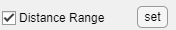
\includegraphics[width=0.6\textwidth]{figuras/Procedimiento_Simulaciones/Radiacion/check_distances2.png}
		\caption{Rango de distancias}
		\label{fig:check_distances}
	\end{subfigure}
	\hfill
	\begin{subfigure}[b]{0.48\textwidth}
		\centering
			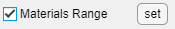
\includegraphics[width=0.6\textwidth]{figuras/Procedimiento_Simulaciones/Radiacion/check_materials2.png}
		\caption{Rango de materiales}
		\label{fig:check_materials}
	\end{subfigure}
	\caption{(\subref{fig:check_distances}) Casilla para la selección de la opción de simular un rango de distancias. (\subref{fig:check_materials}) Casilla para la selección de la opción de simular una combinación de materiales.}%
	\label{fig:checkboxes}%
	\end{figure}
	\item Hacer clic en el \textbf{set} de \textbf{Materials Range}.
	\item Seleccionar los materiales para el emisor (UpFace) y la célula (DownFace), y hacer clic en aceptar (figura \ref{fig:set_materials}).
	\item Hacer clic en el \textbf{set} de \textbf{Distance Range}.	
	\item Seleccionar el rango de distancias a simular de 100 a 1000 o seleccionar la casilla \textbf{Full Range} y hacer clic en aceptar (figura \ref{fig:set_distances}).%% Figuras de las ventanas para los SETs
	\begin{figure}[H]%
	\begin{subfigure}[b]{0.48\textwidth}
		\centering
			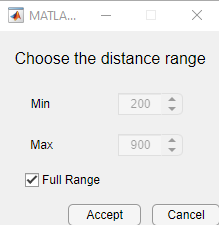
\includegraphics[width=0.6\textwidth]{figuras/Procedimiento_Simulaciones/Radiacion/set_distances_fullrange.png}
		\caption{Set de distancias}
		\label{fig:set_distances}
	\end{subfigure}
	\hfill
	\begin{subfigure}[b]{0.48\textwidth}
		\centering
			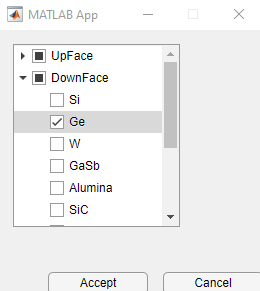
\includegraphics[width=0.6\textwidth]{figuras/Procedimiento_Simulaciones/Radiacion/set_materilas2.png}
		\caption{Set de materiales}
		\label{fig:set_materials}
	\end{subfigure}
	\caption{(\subref{fig:set_distances}) Ventana para la selección del rango de distancias a simular. (\subref{fig:set_materials}) Ventana para la selección de las combinaciones de materiales a simula, siendo \textbf{UpFace} el emisor y \textbf{DownFace} la célula.}%
	\label{fig:sets}%
	\end{figure}
	\item Asegurar que la temperatura del emisor sea la deseada.
	\item Hacer clic en el botón \textbf{Calculate} para ejecutar la simulación.
	\item Esperar que el indicador de estado pase de \textit{Running...}, color rojo del indicador (figura \ref{fig:indicador_Running}), a \textit{StdBy}, color verde del indicador (figura \ref{fig:indicador_StdBy}), es decir, esperar que termine la simulación.
	%% figuras de estados
	\begin{figure}[H]
	\centering
	%% Figura 1
	\begin{subfigure}[b]{0.3\textwidth}
	\centering
	
\includegraphics[width=\textwidth]{figuras/Procedimiento_Simulaciones/Radiacion/estado_changed}%
	\caption{Changed}%
	\label{fig:indicador_Changed}%
	\end{subfigure}
	\hfill
	%% Figura 2
	\begin{subfigure}[b]{0.3\textwidth}
	\centering
	
\includegraphics[width=\textwidth]{figuras/Procedimiento_Simulaciones/Radiacion/estado_running}%
	\caption{Running}%
	\label{fig:indicador_Running}%
	\end{subfigure}
	\hfill
	%% Figura 3
	\begin{subfigure}[b]{0.3\textwidth}
	\centering
	
\includegraphics[width=0.9\textwidth]{figuras/Procedimiento_Simulaciones/Radiacion/estado_stdby}%
	\caption{StdBy}%
	\label{fig:indicador_StdBy}%
	\end{subfigure}
	\hfill
	\caption{Indicadores del estado actual del sistema. (\subref{fig:indicador_Changed}) Indicador del estado \textbf{Changed} o estado de cambio, se activa cuando se produce algún cambio en los datos seleccionados para simular. (\subref{fig:indicador_Running}) Indicador del estado \textbf{Running} o corriendo, se activa cuando estando en el estado \textbf{Changed} se hace clic al botón \textbf{Calculate} y corre la simulación. (\subref{fig:indicador_StdBy}) Indicador del estado \textbf{StdBy}, se activa cuando termina la simulación, avisando que está a la espera de algún cambio.}
	\label{fig:indicadorLED}
	\end{figure}
	%% Se acaba la figura
	\item Ir a la pestaña de \textbf{Potencia}.
	\item Introducir el rango de longitudes de onda para calcular la potencia por unidad de área, siendo elegido desde el mínimo hasta 1.8 $\mu m$ que es el rango de longitudes de onda que absorbe la célula de Ge (figura \ref{fig:graficar_ejemplo2}).
	\item Hacer clic en el botón \textbf{Graph} para calcular y graficar las potencias (figura \ref{fig:graficar_ejemplo2}).
\end{enumerate}
%% Graficas de la pestaña de potencia
\begin{figure}[H]
	\centering
	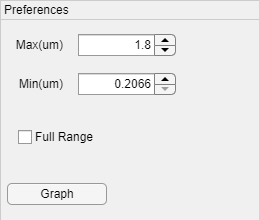
\includegraphics[width=0.30\textwidth]{figuras/Procedimiento_Simulaciones/Radiacion/graficar_ejemplo2.png}
	\caption{Preferencias para el cálculo de la potencia}
	\label{fig:graficar_ejemplo2}
\end{figure}
%% Guardar resultados
El procedimiento seguido en este trabajo se encuentra detallado paso a paso en el Apéndice \ref{ch:procedimientosSimRad}. Para la extracción de los datos obtenidos de potencia por unidad de área se hace clic sobre el botón de \textbf{guardar} (figura \ref{fig:SaveButton_Cut}) estando en la pestaña \textbf{Potencia}, para guardar la potencia radiada se hace clic del botón de \textbf{guardar} estando en la pestaña de \textbf{Potencia Radiada} y para guardar todos los datos se hace clic sobre el botón de \textbf{guardar todos} (figura \ref{fig:SaveAllicon}).
\begin{figure}[H]
	\centering
	\begin{subfigure}[b]{0.48\textwidth}
		\centering
		
\includegraphics[width=0.4\textwidth]{figuras/Procedimiento_Simulaciones/Radiacion/SaveButton_Cut.jpg}
		\caption{Botón de guardar actual}
		\label{fig:SaveButton_Cut}
	\end{subfigure}
  \hfill
	\begin{subfigure}[b]{0.48\textwidth}
		\centering
			
\includegraphics[width=0.40\textwidth]{figuras/Procedimiento_Simulaciones/Radiacion/SaveAllicon.jpg}
		\caption{Botón de guardar todos los resultados}
		\label{fig:SaveAllicon}
	\end{subfigure}
	\caption{(\subref{fig:SaveButton_Cut}) Botón de guardar los resultados obtenidos de los cálculos o la simulación, dependiendo de la pestaña que se encuentre el usuario de la calculadora de campo cercano. (\subref{fig:SaveAllicon}) Botón de guardar todos los resultados obtenidos de los cálculos y simulación.}
	\label{fig:saveButtons}
\end{figure}
%%%%%%%%%%%%     Conducción térmica
\subsection{Para la conducción térmica}
Las simulaciones de transmisión de calor por conducción se realizaron todas en CFD, existiendo unos 10 casos para cada combinación de materiales y resistencias de contacto, para cada uno de ellos se sigue un mismo conjunto de pasos. \\\\
Primero hay que crear el modelo 3D de cada componente del sistema TPV a simular, siendo cada uno de ellos es un prisma de sección cuadrada. El nano-espaciador tiene de base un cuadrado de lado 3 $\mu m$ y de altura variable $h$, el emisor y la célula tiene el mismo modelo 3D, con base cuadrada de 1mm de lado con 0.2mm de altura. Para el cálculo de las longitudes del modelo 3D se utiliza la ecuación \eqref{eq:relacion_longitud}.
%%% MODELADO 3D
\subsubsection{Procedimiento modelado 3D}
El procedimiento seguido para la obtención de los modelos 3D en Inventor y la creación del modelo de simulación inicial para cada altura del nano-espaciador es:
\begin{enumerate}
	\item Crear las bases cuadradas con la longitud de lado respectiva, 10m para emisor o célula y 3cm para el nano-espaciador en la escala del modelo 3D en Inventor. 
	\item Extrudir el prisma la longitud correspondiente, 2m para el emisor/célula y $h_0$ para el nano-espaciador, siendo $h$ un valor inicial cualquier en el rango de 1mm a 10mm.
	\item Crear un ensamblaje de emisor-espaciador-célula, estando la base del nano-espaciador en el centro de las bases de los otros dos componentes (figura \ref{fig:modelado3D}).
	%% PASOS PARA EL ENSAMBLAJE
	\begin{enumerate}
		\item Agregar el nano-espaciador y los dos prismas de 10m de lado.
		\item Renombrar los prismas de 10m de lado, una siendo emisor y la otra célula, para así diferenciarlas.
		\item Obtener el centro de la cara superior de la célula, mediante un dibujo con dos rectas secantes que van de una esquina a otra (figura \ref{fig:modelado3D_centro_cerca}).
		\item Aplicar una restricción con la opción \textbf{Mate} de separación nula entre la cara inferior del nano-espaciador con el centro de la cara superior de la célula,es decir, las caras entran en contacto si la distancia de separación es nula (figura \ref{fig:modelado3D_centro_cerca}).
		\item Aplicar una restricción \textbf{Mate} de separación nula entre la cara inferior del emisor y la cara superior del nano-espaciador.
		\item Aplicar una restricción \textbf{Flush} de separación nula a una cara lateral del emisor y una cara lateral de la célula.
		\item Repetir el paso anterior para las caras conjuntas, siendo el resultado final el de la figura \ref{fig:modelado3D_lejos}.
	\end{enumerate}
\begin{figure}[H]
	\centering
	\begin{subfigure}[b]{0.3\textwidth}
		\centering
			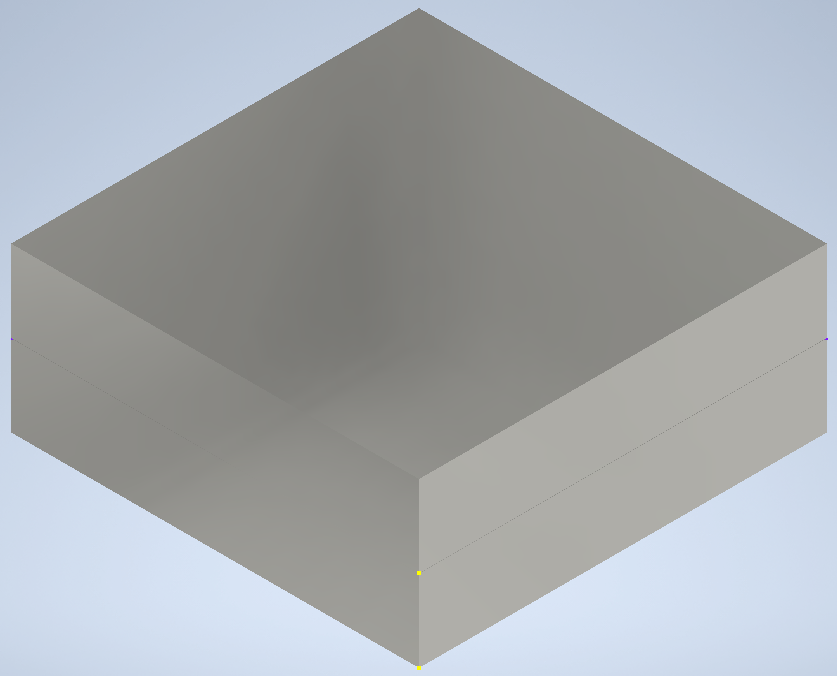
\includegraphics[width=1.00\textwidth]{figuras/Procedimiento_Simulaciones/Conduccion/modelado3D_lejos.png}
		\caption{Vista global TPV}
		\label{fig:modelado3D_lejos}
	\end{subfigure}
	\hfill
	\begin{subfigure}[b]{0.3\textwidth}
		\centering
			
\includegraphics[width=1.00\textwidth]{figuras/Procedimiento_Simulaciones/Conduccion/modelado3D_cerca.png}
		\caption{Vista cerca TPV}
		\label{fig:modelado3D_cerca}
	\end{subfigure}
	\hfill
	\begin{subfigure}[b]{0.3\textwidth}
		\centering
			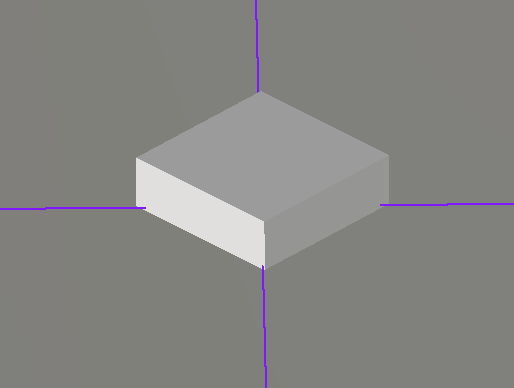
\includegraphics[width=1.00\textwidth]{figuras/Procedimiento_Simulaciones/Conduccion/modelado3D_centro_cerca.png}
		\caption{Vista cerca nano-espaciador}
		\label{fig:modelado3D_centro_cerca}
	\end{subfigure}
	\caption{Vistas del sistema TPV. (\subref{fig:modelado3D_lejos}) Vista de lejos del sistema completo de la TPV. (\subref{fig:modelado3D_cerca}) Vista del sistema TPV de cerca desde un borde. (\subref{fig:modelado3D_centro_cerca}) Vista del nano-espaciador colocado sobre el centro de una cara de la célula.}
	\label{fig:modelado3D}
\end{figure}
	\item Guardar el ensamblaje.
	\item Usar el \textbf{Active Model Assessment Tool}, que se encuentra en la pestaña de simulaciones, para generar el modelo o estudio de simulación de CFD\label{itm:pasoIniIterativo_Modelado3D}.
	\item Al abrirse CFD hacer clic en \textit{Transfer to Set Up}, dar un nombre y lanzar.
	\item Guardar el modelo o estudio de CFD \label{itm:pasoFin_Modelado3D}.
	\item Ir al ensamblaje en Inventor.
	\item Hacer clic derecho sobre el ícono del objeto correspondiente al nano-espaciador en el panel \textbf{model} y hacer clic en editar.
	\item Hacer clic derecho sobre la extrusión y seleccionar la opción de editar característica (\textbf{Edit Feature}).
	\item Modificar la altura del nano-espaciador y al terminar hacer clic en \textbf{Return} \label{itm:pasoFinIterativo_Modelado3D}.
	\item Repetir desde el paso \ref{itm:pasoIniIterativo_Modelado3D} al \ref{itm:pasoFinIterativo_Modelado3D}, excepto en la última iteración que es hasta el paso \ref{itm:pasoFin_Modelado3D}, incluido.
\end{enumerate} 

\subsubsection{Procedimiento simulación CFD}
%%%  PROCEDIMIENTO CFD
El procedimiento a seguir para cada modelo de la simulación de transmisión de calor por conducción en CFD es el siguiente:
\begin{enumerate}
	\item Abrir el modelo o estudio correspondiente de simulación en CFD.
	\item Seleccionar el emisor y cambiar el material por defecto por el que se va a simular a escala.
	\item Seleccionar el entorno del material del emisor como variable.
	\item Seleccionar la célula y cambiar el material por defecto por el que se va a simular a escala.
	\item Seleccionar el entorno del material de la célula como variable.
	\item Hacer zoom sobre el nano-espaciador, seleccionarlo y cambiar el material por defecto por el $SiO_2$ a escala.
	\item Seleccionar el entorno del material del nano-espaciador como variable.
	\item \textbf{En el caso que la resistencia de contacto no sea nula:}
	\begin{enumerate}
		\item Esconder el emisor.
		\item Seleccionar el selector de superficies.
		\item Seleccionar la superficie superior del nano-espaciador, es decir, la superficie que hace contacto con el emisor.
		\item Cambiar el material por defecto por la resistencia de contacto a escala.
		\item Seleccionar el selector de volúmenes.
		\item Mostrar el emisor.
	\end{enumerate}
	%% PANEL DE HERRAMIENTAS
	\begin{figure}[H]
	\centering
	\begin{subfigure}[b]{0.48\textwidth}
		\centering
			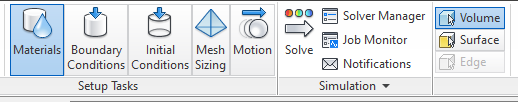
\includegraphics[width=0.9\textwidth]{figuras/Procedimiento_Simulaciones/Conduccion/paneles.png}
		\caption{Panel principal}
		\label{fig:paneles}
		\end{subfigure}
		\hfill
		\begin{subfigure}[b]{0.48\textwidth}
			\centering
			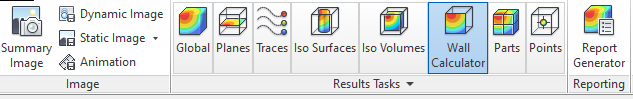
\includegraphics[width=0.9\textwidth]{figuras/Procedimiento_Simulaciones/Conduccion/paneles_resultados.png}
			\caption{Panel de resultados}
			\label{fig:paneles_resultados}
		\end{subfigure}
		\caption{(\subref{fig:paneles}) Panel de las herramientas utilizadas para aplicar materiales, condiciones de contorno, lanzar simulaciones, seleccionar el selector de superficies y volúmenes. (\subref{fig:paneles_resultados}) Paneles de las herramientas utilizadas para la extracción de resultados de las simulaciones de transmisión de calor por conducción.}
		\label{fig:paneles_CFD}
	\end{figure}
	\item Seleccionar la cara superior del emisor y agregar como condición de contorno una temperatura constante de 800\textdegree C.
	\item Seleccionar la cara inferior de la célula y agregar como condición de contorno una temperatura constante de 25\textdegree C.
	\item Seleccionar la función de mallado.
	\item Aplicar un mallado de tamaño de 0.01 o más al nano-espaciador, el valor del mallado varía según la altura del nano-espaciador, aumentando al aumentar la altura del nano-espciador (figura \ref{fig:mallados_metodos}).
	\item Aplicar un mallado de tamaño entre 40 y 60 a los demás componentes de la TPV.
	%%% FIGURAS DE MALLADO
	\begin{figure}[H]
	\centering
	\begin{subfigure}[b]{0.3\textwidth}
		\centering
			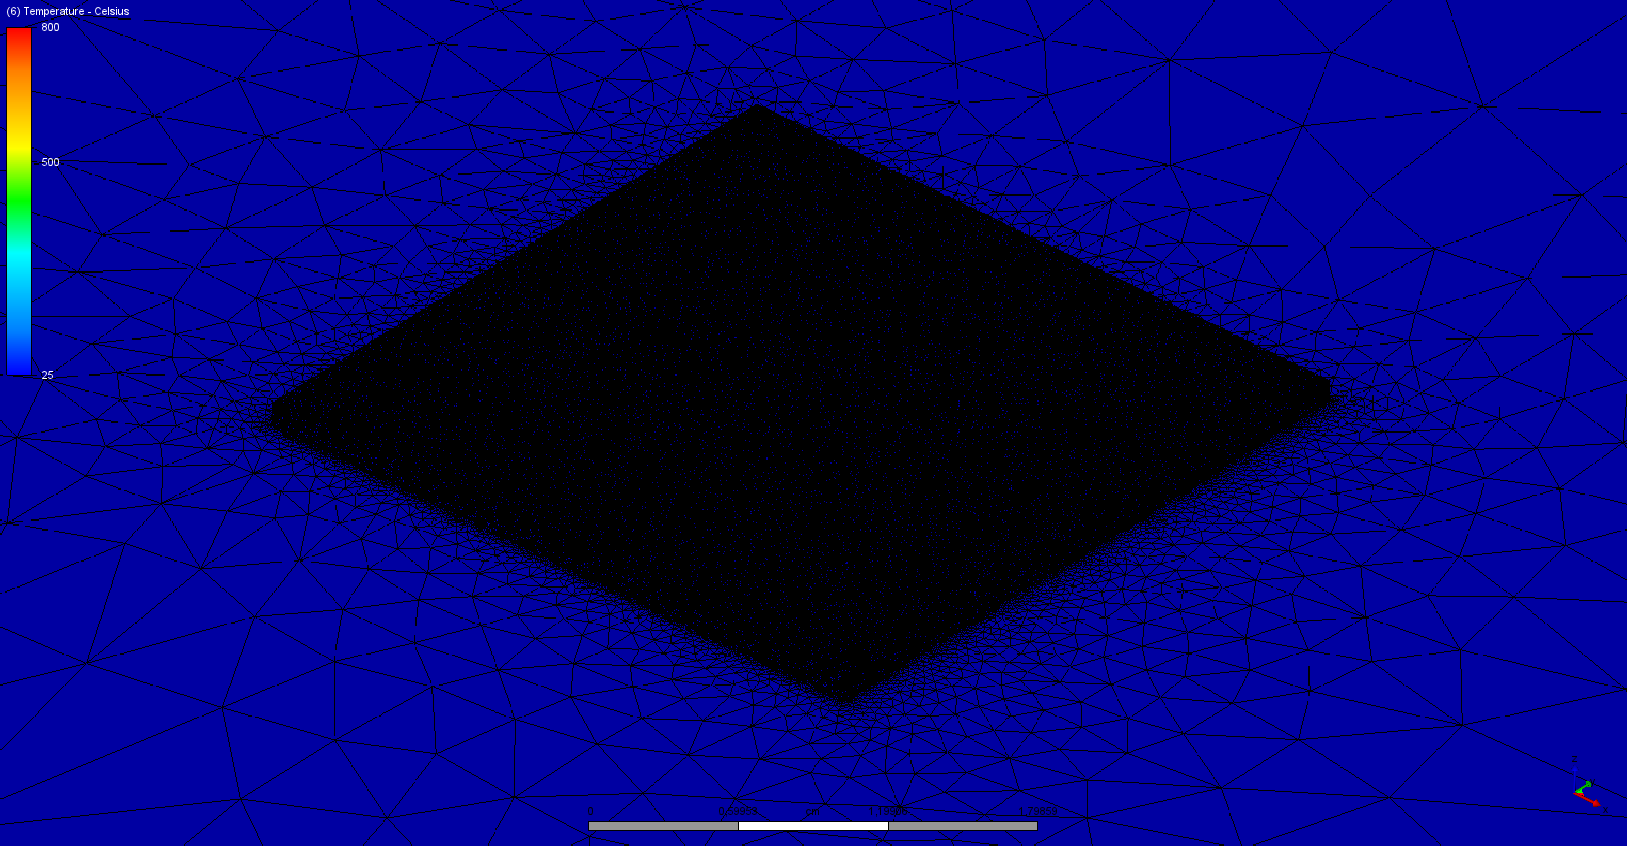
\includegraphics[width=1.00\textwidth]{figuras/Procedimiento_Simulaciones/Conduccion/mallado_100.png}
		\caption{Mallado del nano-espaciador de 100nm}
		\label{fig:mallado_100_metodos}
	\end{subfigure}
	\hfill
	\begin{subfigure}[b]{0.3\textwidth}
		\centering
			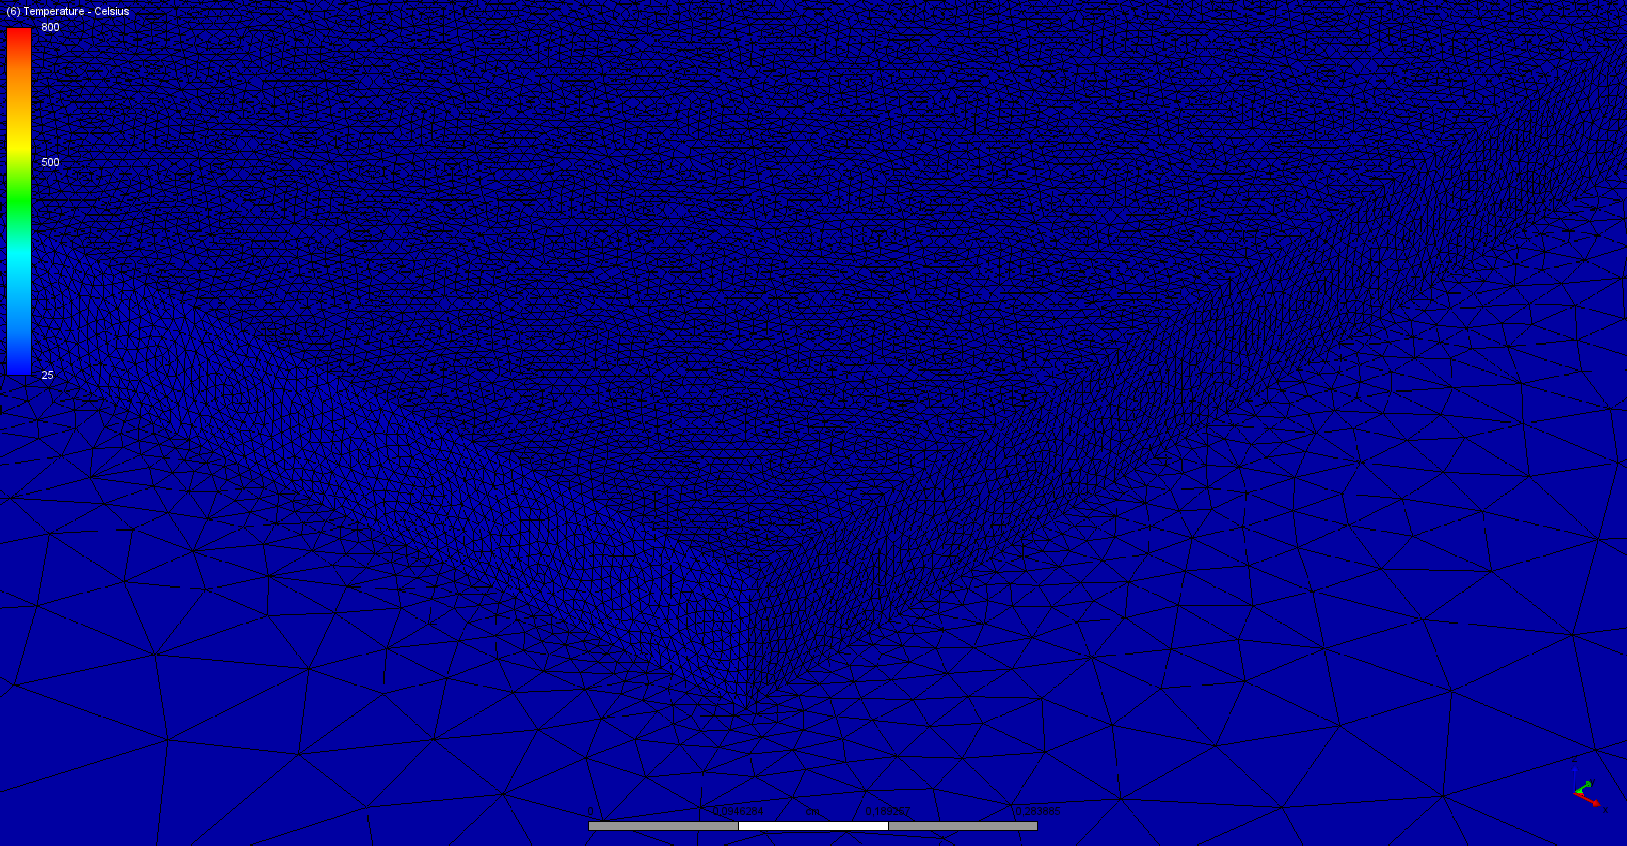
\includegraphics[width=1.00\textwidth]{figuras/Procedimiento_Simulaciones/Conduccion/mallado_100_cerca.png}
		\caption{Mallado del nano-espaciador de 100nm de cerca}
		\label{fig:mallado_100_cerca_metodos}
	\end{subfigure}
	\hfill
	\begin{subfigure}[b]{0.3\textwidth}
		\centering
			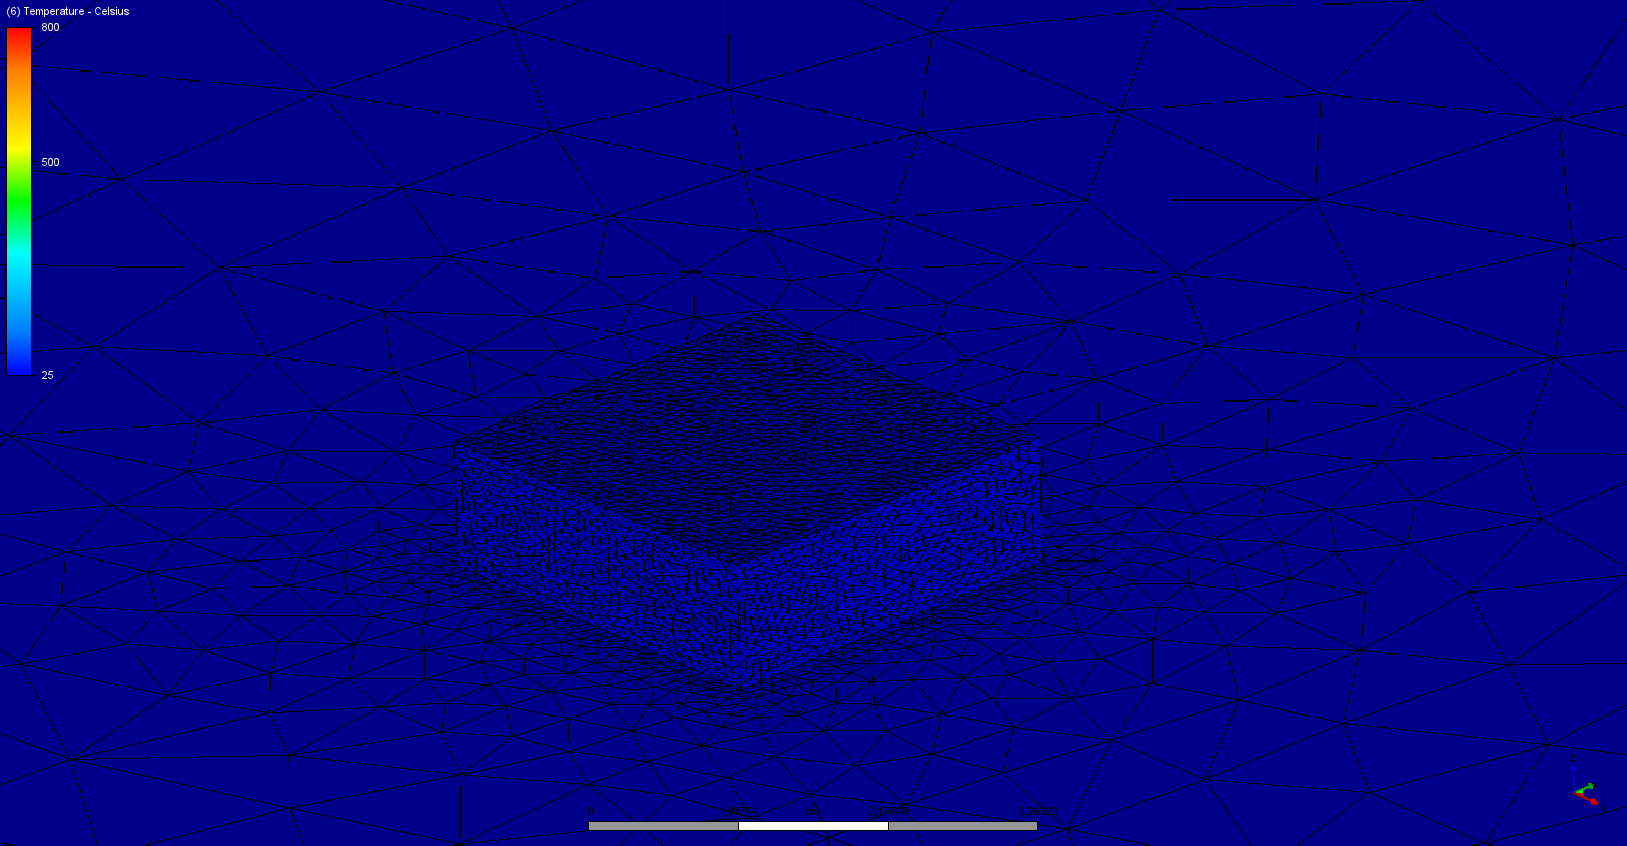
\includegraphics[width=1.00\textwidth]{figuras/Procedimiento_Simulaciones/Conduccion/mallado_1000.png}
		\caption{Mallado del nano-espaciador de 1000nm}
		\label{fig:mallado_1000_cerca_metodos}
	\end{subfigure}
	\caption{(\subref{fig:mallado_100_metodos}) Mallado del nano-espaciador de 100nm, con tamaño de malla de 0.01. (\subref{fig:mallado_100_cerca_metodos}) Mallado del nano-espaciador de 100nm visto de cerca. (\subref{fig:mallado_1000_cerca_metodos}) Mallado del nano-espaciador de 1000nm, con tamaño de malla de 0.1.}
	\label{fig:mallados_metodos}
\end{figure} 
%%% CONTINUA ENUMERACION
	\item Hacer clic en \textbf{Solve} (figura \ref{fig:paneles}).
	\item Seleccionar en la pestaña \textbf{Physics} la casilla de \textbf{Heat transfer} (\ref{fig:physics_panel}) .
	\item Ir a la pestaña \textbf{Control} (figura \ref{fig:control_panel}).
	\item Poner el guardado de los resultados de la simulación a la mitad del número de iteraciones.
	\item Hacer unas 10 a 14 iteraciones asegurándose que continua desde la iteración cero.
	\item Correr la simulación dando click al botón de \textbf{Solve} dentro de la ventana del lanzar la simulación.
	%%% VENTANA DEL SOLVER
	\begin{figure}[H]
		\centering
		\begin{subfigure}[b]{0.48\textwidth}
			\centering
			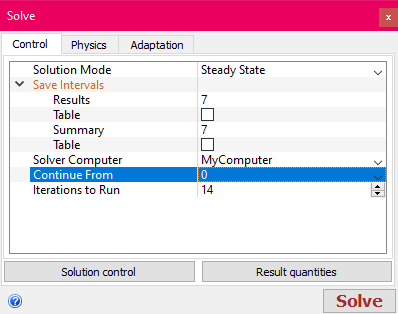
\includegraphics[width=0.8\textwidth]{figuras/Procedimiento_Simulaciones/Conduccion/control_panel.png}
			\caption{panel de control del solver}
			\label{fig:control_panel}
		\end{subfigure}
	  \hfill
		\begin{subfigure}[b]{0.48\textwidth}
			\centering
			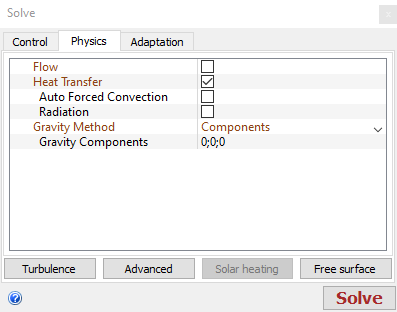
\includegraphics[width=0.8\textwidth]{figuras/Procedimiento_Simulaciones/Conduccion/physics_panel.png}
			\caption{panel de la física del solver}
			\label{fig:physics_panel}
		\end{subfigure}
		\caption{(\subref{fig:control_panel}) Panel de control de la ventana del Solver.(\subref{fig:physics_panel}) Panel de las propiedades físicas de la ventana del Solver.}
		\label{fig:panels_Solver}
	\end{figure}
	%%    CONTINUA
	\item Esperar a que la simulación termine. Un mensaje aparecerá en la ventana de salidas de que la simulación ha finalizado.
	%% Extracción de los resultados
	\item \textbf{Extraer los datos de la simulación en un archivo CSV}.\label{it:extraerResCFD}
	\begin{enumerate}
		\item Abrir la herramienta \textbf{Wall Calculator} con un clic (figura \ref{fig:paneles_resultados}).
		\item Seleccionar las casillas de potencia y temperatura.
		\item Seleccionar la opción de superficie del \textbf{Model entity selection}.
		\item Seleccionar la superficie superior del emisor y la inferior de la célula, aparecerá los números correspondientes a dichas superficies en el \textbf{Wall Calculator} (figura \ref{fig:ventana_wall_calculator_control}).
		\item Hacer clic en \textbf{Calculate}, esto nos llevará a la pestaña de \textbf{Output}.
		\item Hacer clic en \textbf{Write to file} y guardar el archivo de salida que contiene las potencias y temperaturas medias de las superficies seleccionadas (figura \ref{fig:ventana_wall_calculator_resultados}).
	\end{enumerate}
		%%% VENTANA DEL WALL CALCULATOR
	\begin{figure}[H]
		\centering
		\begin{subfigure}[b]{0.48\textwidth}
			\centering
			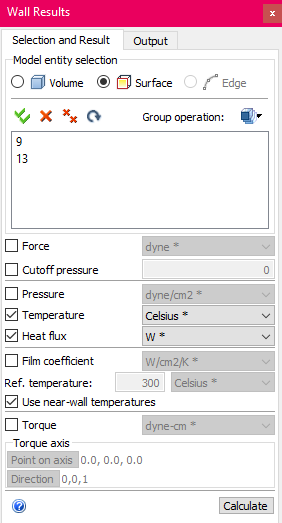
\includegraphics[width=0.6\textwidth]{figuras/Procedimiento_Simulaciones/Conduccion/ventana_wall_calculator.png}
			\caption{Pestaña de selección y resultados.}
			\label{fig:ventana_wall_calculator_control}
		\end{subfigure}
	  \hfill
		\begin{subfigure}[b]{0.48\textwidth}
			\centering
			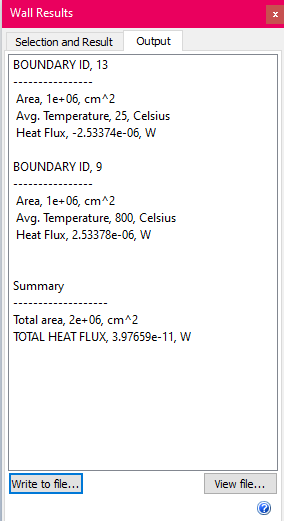
\includegraphics[width=0.6\textwidth]{figuras/Procedimiento_Simulaciones/Conduccion/resultados_conduccion.png}
			\caption{Pestaña de salida.}
			\label{fig:ventana_wall_calculator_resultados}
		\end{subfigure}
		\caption{(\subref{fig:ventana_wall_calculator_control}) Pestaña de selección y resultados del \textbf{Wall Calculator}.(\subref{fig:ventana_wall_calculator_resultados}) Pestaña de salida del \textbf{Wall Calculator}.}
		\label{fig:ventana_wall_calculator}
	\end{figure}
	\item Repetir los pasos anteriores para cada combinación de materiales y resistencias de contacto sin tener que volver a introducir las condiciones de contorno o volver a configurar el mallado.
	\item Repetir los pasos anteriores para cada altura del nano-espaciador.
\end{enumerate}